% Options for packages loaded elsewhere
\PassOptionsToPackage{unicode}{hyperref}
\PassOptionsToPackage{hyphens}{url}
\documentclass[
]{article}
\usepackage{xcolor}
\usepackage{amsmath,amssymb}
\setcounter{secnumdepth}{-\maxdimen} % remove section numbering
\usepackage{iftex}
\ifPDFTeX
  \usepackage[T1]{fontenc}
  \usepackage[utf8]{inputenc}
  \usepackage{textcomp} % provide euro and other symbols
\else % if luatex or xetex
  \usepackage{unicode-math} % this also loads fontspec
  \defaultfontfeatures{Scale=MatchLowercase}
  \defaultfontfeatures[\rmfamily]{Ligatures=TeX,Scale=1}
\fi
\usepackage{lmodern}
\ifPDFTeX\else
  % xetex/luatex font selection
\fi
% Use upquote if available, for straight quotes in verbatim environments
\IfFileExists{upquote.sty}{\usepackage{upquote}}{}
\IfFileExists{microtype.sty}{% use microtype if available
  \usepackage[]{microtype}
  \UseMicrotypeSet[protrusion]{basicmath} % disable protrusion for tt fonts
}{}
\makeatletter
\@ifundefined{KOMAClassName}{% if non-KOMA class
  \IfFileExists{parskip.sty}{%
    \usepackage{parskip}
  }{% else
    \setlength{\parindent}{0pt}
    \setlength{\parskip}{6pt plus 2pt minus 1pt}}
}{% if KOMA class
  \KOMAoptions{parskip=half}}
\makeatother
\usepackage{longtable,booktabs,array}
\newcounter{none} % for unnumbered tables
\usepackage{calc} % for calculating minipage widths
% Correct order of tables after \paragraph or \subparagraph
\usepackage{etoolbox}
\makeatletter
\patchcmd\longtable{\par}{\if@noskipsec\mbox{}\fi\par}{}{}
\makeatother
% Allow footnotes in longtable head/foot
\IfFileExists{footnotehyper.sty}{\usepackage{footnotehyper}}{\usepackage{footnote}}
\makesavenoteenv{longtable}
\usepackage{graphicx}
\makeatletter
\newsavebox\pandoc@box
\newcommand*\pandocbounded[1]{% scales image to fit in text height/width
  \sbox\pandoc@box{#1}%
  \Gscale@div\@tempa{\textheight}{\dimexpr\ht\pandoc@box+\dp\pandoc@box\relax}%
  \Gscale@div\@tempb{\linewidth}{\wd\pandoc@box}%
  \ifdim\@tempb\p@<\@tempa\p@\let\@tempa\@tempb\fi% select the smaller of both
  \ifdim\@tempa\p@<\p@\scalebox{\@tempa}{\usebox\pandoc@box}%
  \else\usebox{\pandoc@box}%
  \fi%
}
% Set default figure placement to htbp
\def\fps@figure{htbp}
\makeatother
\setlength{\emergencystretch}{3em} % prevent overfull lines
\providecommand{\tightlist}{%
  \setlength{\itemsep}{0pt}\setlength{\parskip}{0pt}}
\usepackage[margin=2.5cm]{geometry}
\usepackage{float}
\usepackage{bookmark}
\IfFileExists{xurl.sty}{\usepackage{xurl}}{} % add URL line breaks if available
\urlstyle{same}
\hypersetup{
  hidelinks,
  pdfcreator={LaTeX via pandoc}}

\author{}
\date{}

\begin{document}

\section{PGI-RC Correction: Results}

\subsection{Corrected inequality of opportunity estimates}

In MoBa, Howe's correction is the preferred one, because it is based on the same data and includes both between and within family SNP heritability estimates. In WLS, the choice is less clear, because Becker's correction is based on WLS data, but within family SNP heritability is inferred from Howe et al. We could keep Howe's correction in WLS for internal consistency of between and within SNP heritability.

The correction substantially reduces IOLib --- because the noisy PGI
currently over-attributes variance to shared family environment --- and
modestly increases IORad through within-family variance. The gap roughly
doubles when corrections are applied. The effect size of the correction
is consistent with Becker et al.~(2021), see Table 3 in their paper for
an example of correction.


\begin{figure}[ht]
\centering
\pandocbounded{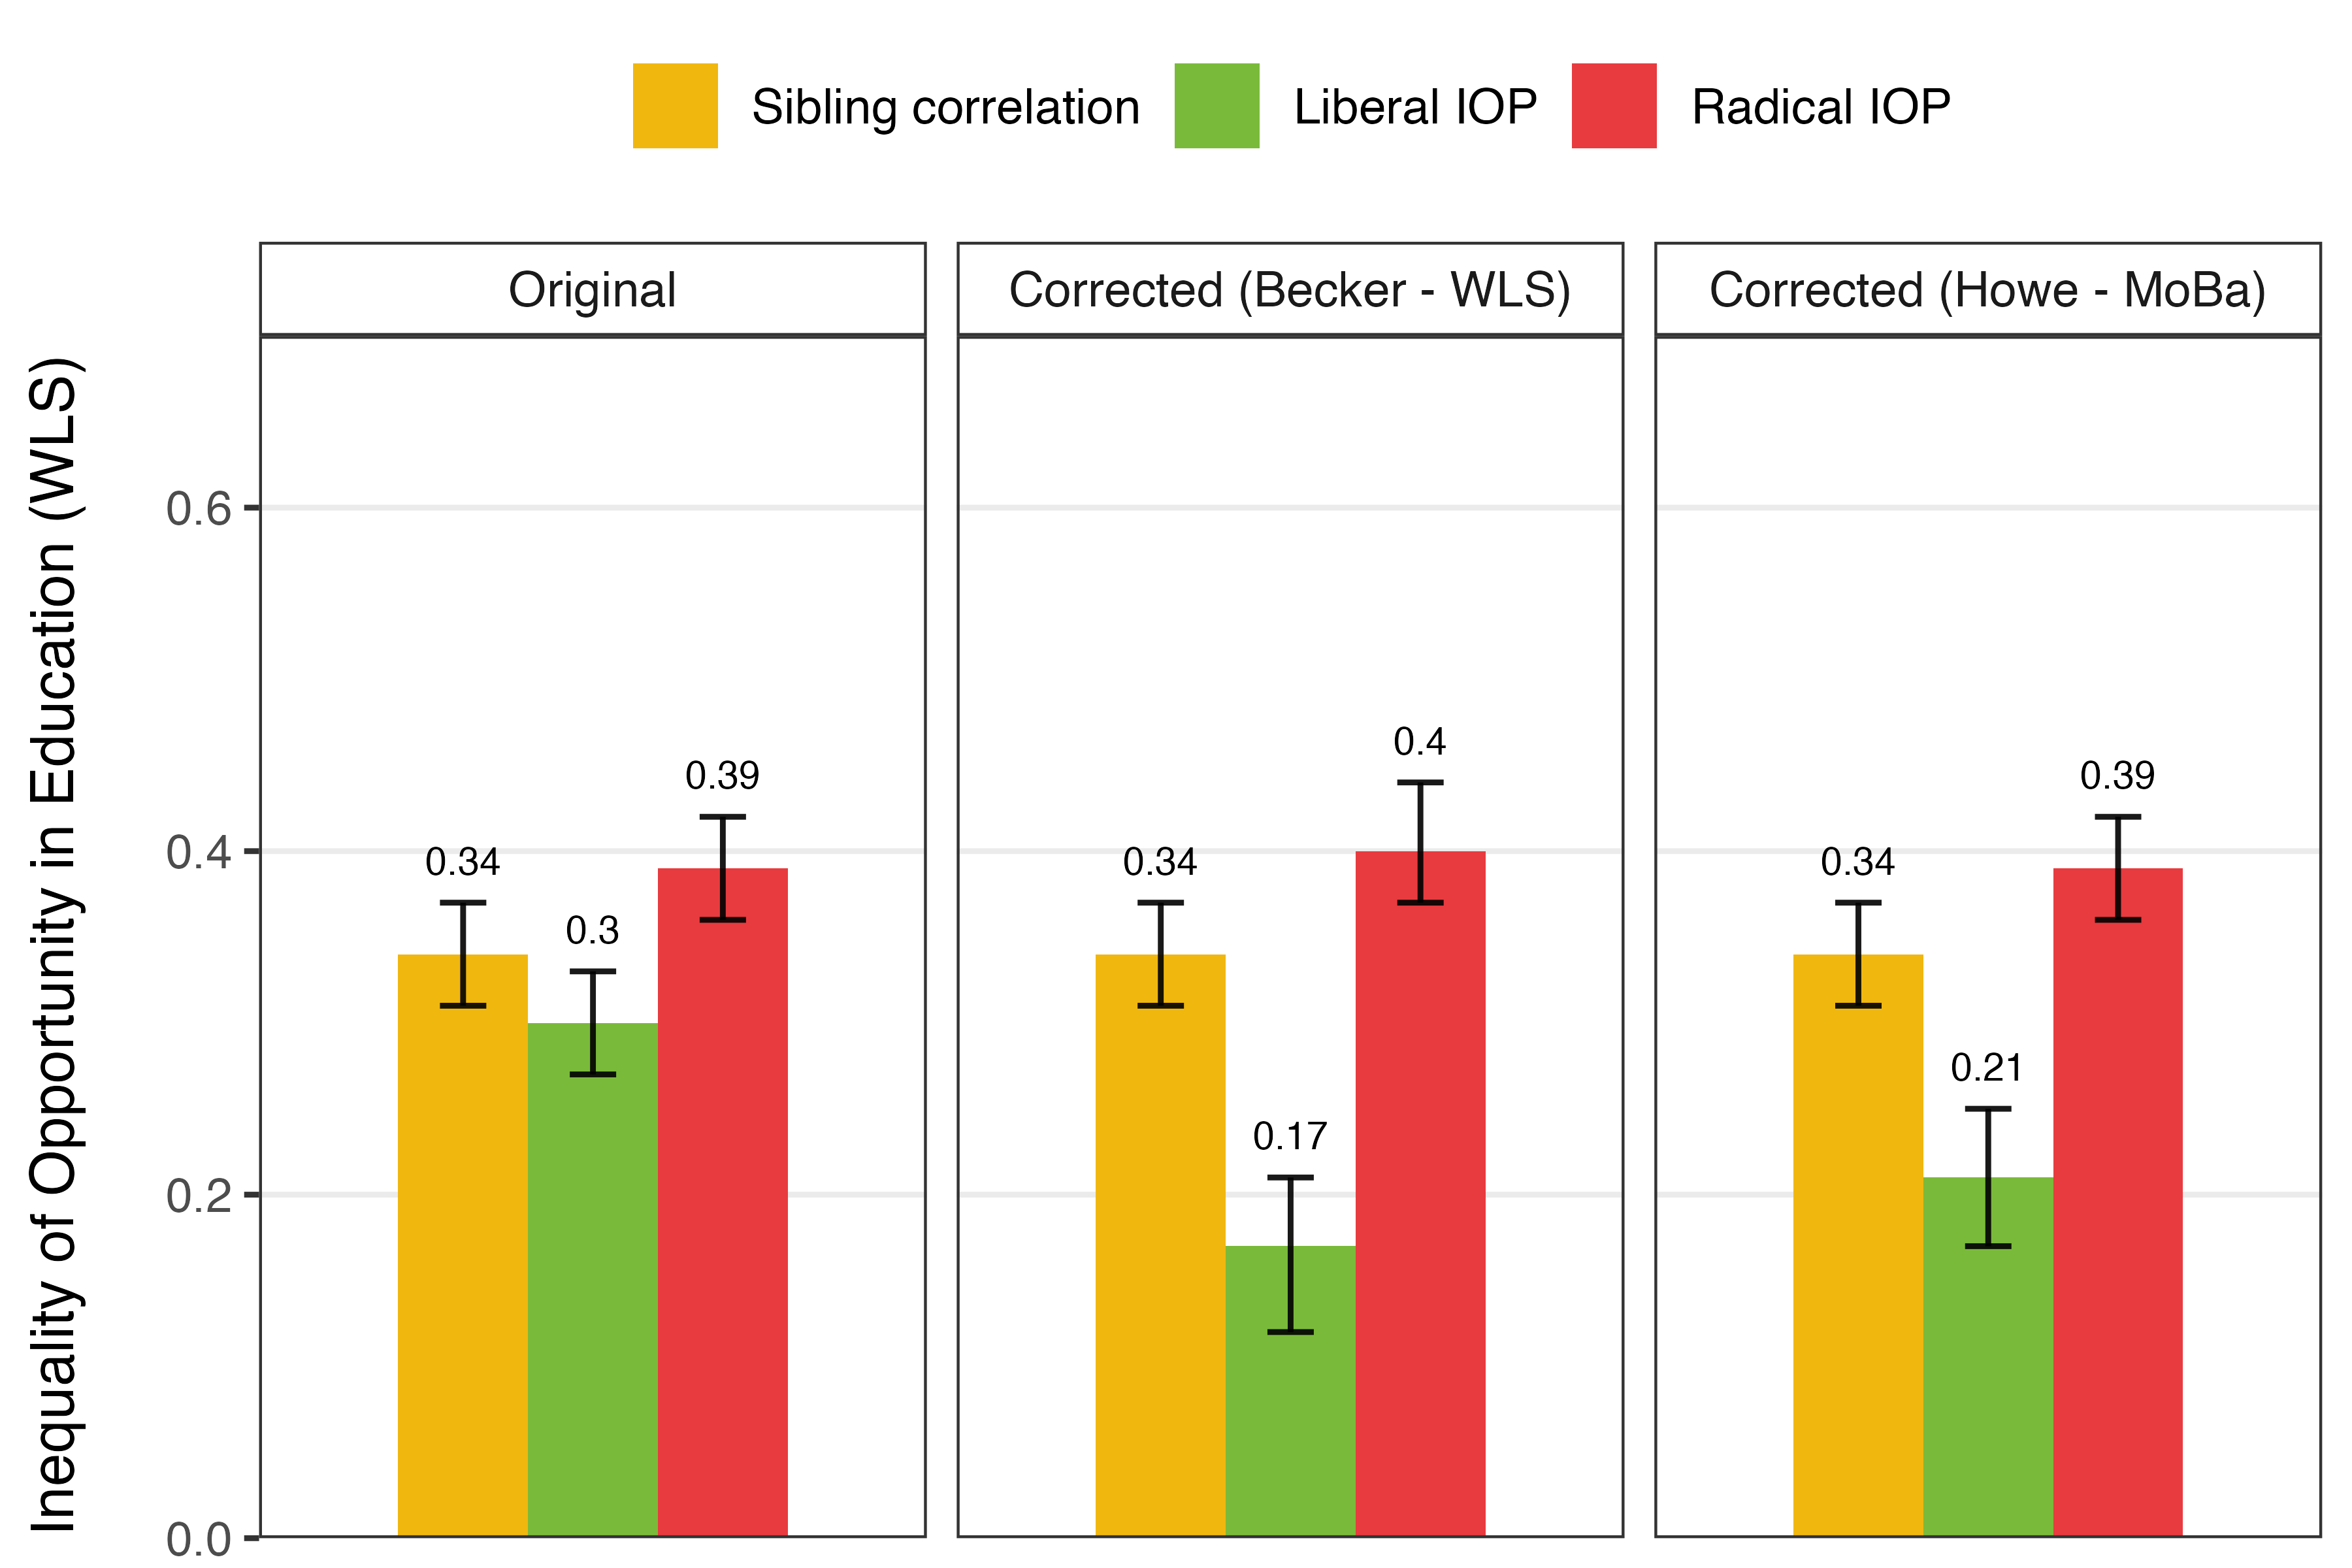
\includegraphics[keepaspectratio,alt={full plot}]{plots/PGI_RC_correction_WLS.png}}
\caption{WLS: corrected indices}
\end{figure}

\begin{table}[H]
\begin{tabular}{@{}lcccccccc@{}}
\toprule
 & $h^2_\text{between}$ & $h^2_\text{within}$ & $\rho_\text{between}$ & $\rho_\text{within}$ & Sibcorr & IOLib & IORad & Gap \\
\midrule
Original & --- & --- & --- & --- & 0.34 & 0.30 & 0.39 & 0.09 \\
Corrected (Becker -- WLS) & 0.119 & 0.053 & 1.939 & 1.255 & 0.34 & 0.17 & 0.40 & 0.23 \\
Corrected (Howe -- MoBa) & 0.090 & 0.040 & 1.686 & 1.091 & 0.34 & 0.21 & 0.39 & 0.18 \\
\bottomrule
\end{tabular}
\end{table}

\emph{WLS data parameters: \(R^2_\text{between} = 0.094\),
\(R^2_\text{within} = 0.051\), ICC \(= 0.337\),
\(R^2_\text{pop} = 0.065\).}



\begin{figure}[ht]
\centering
\pandocbounded{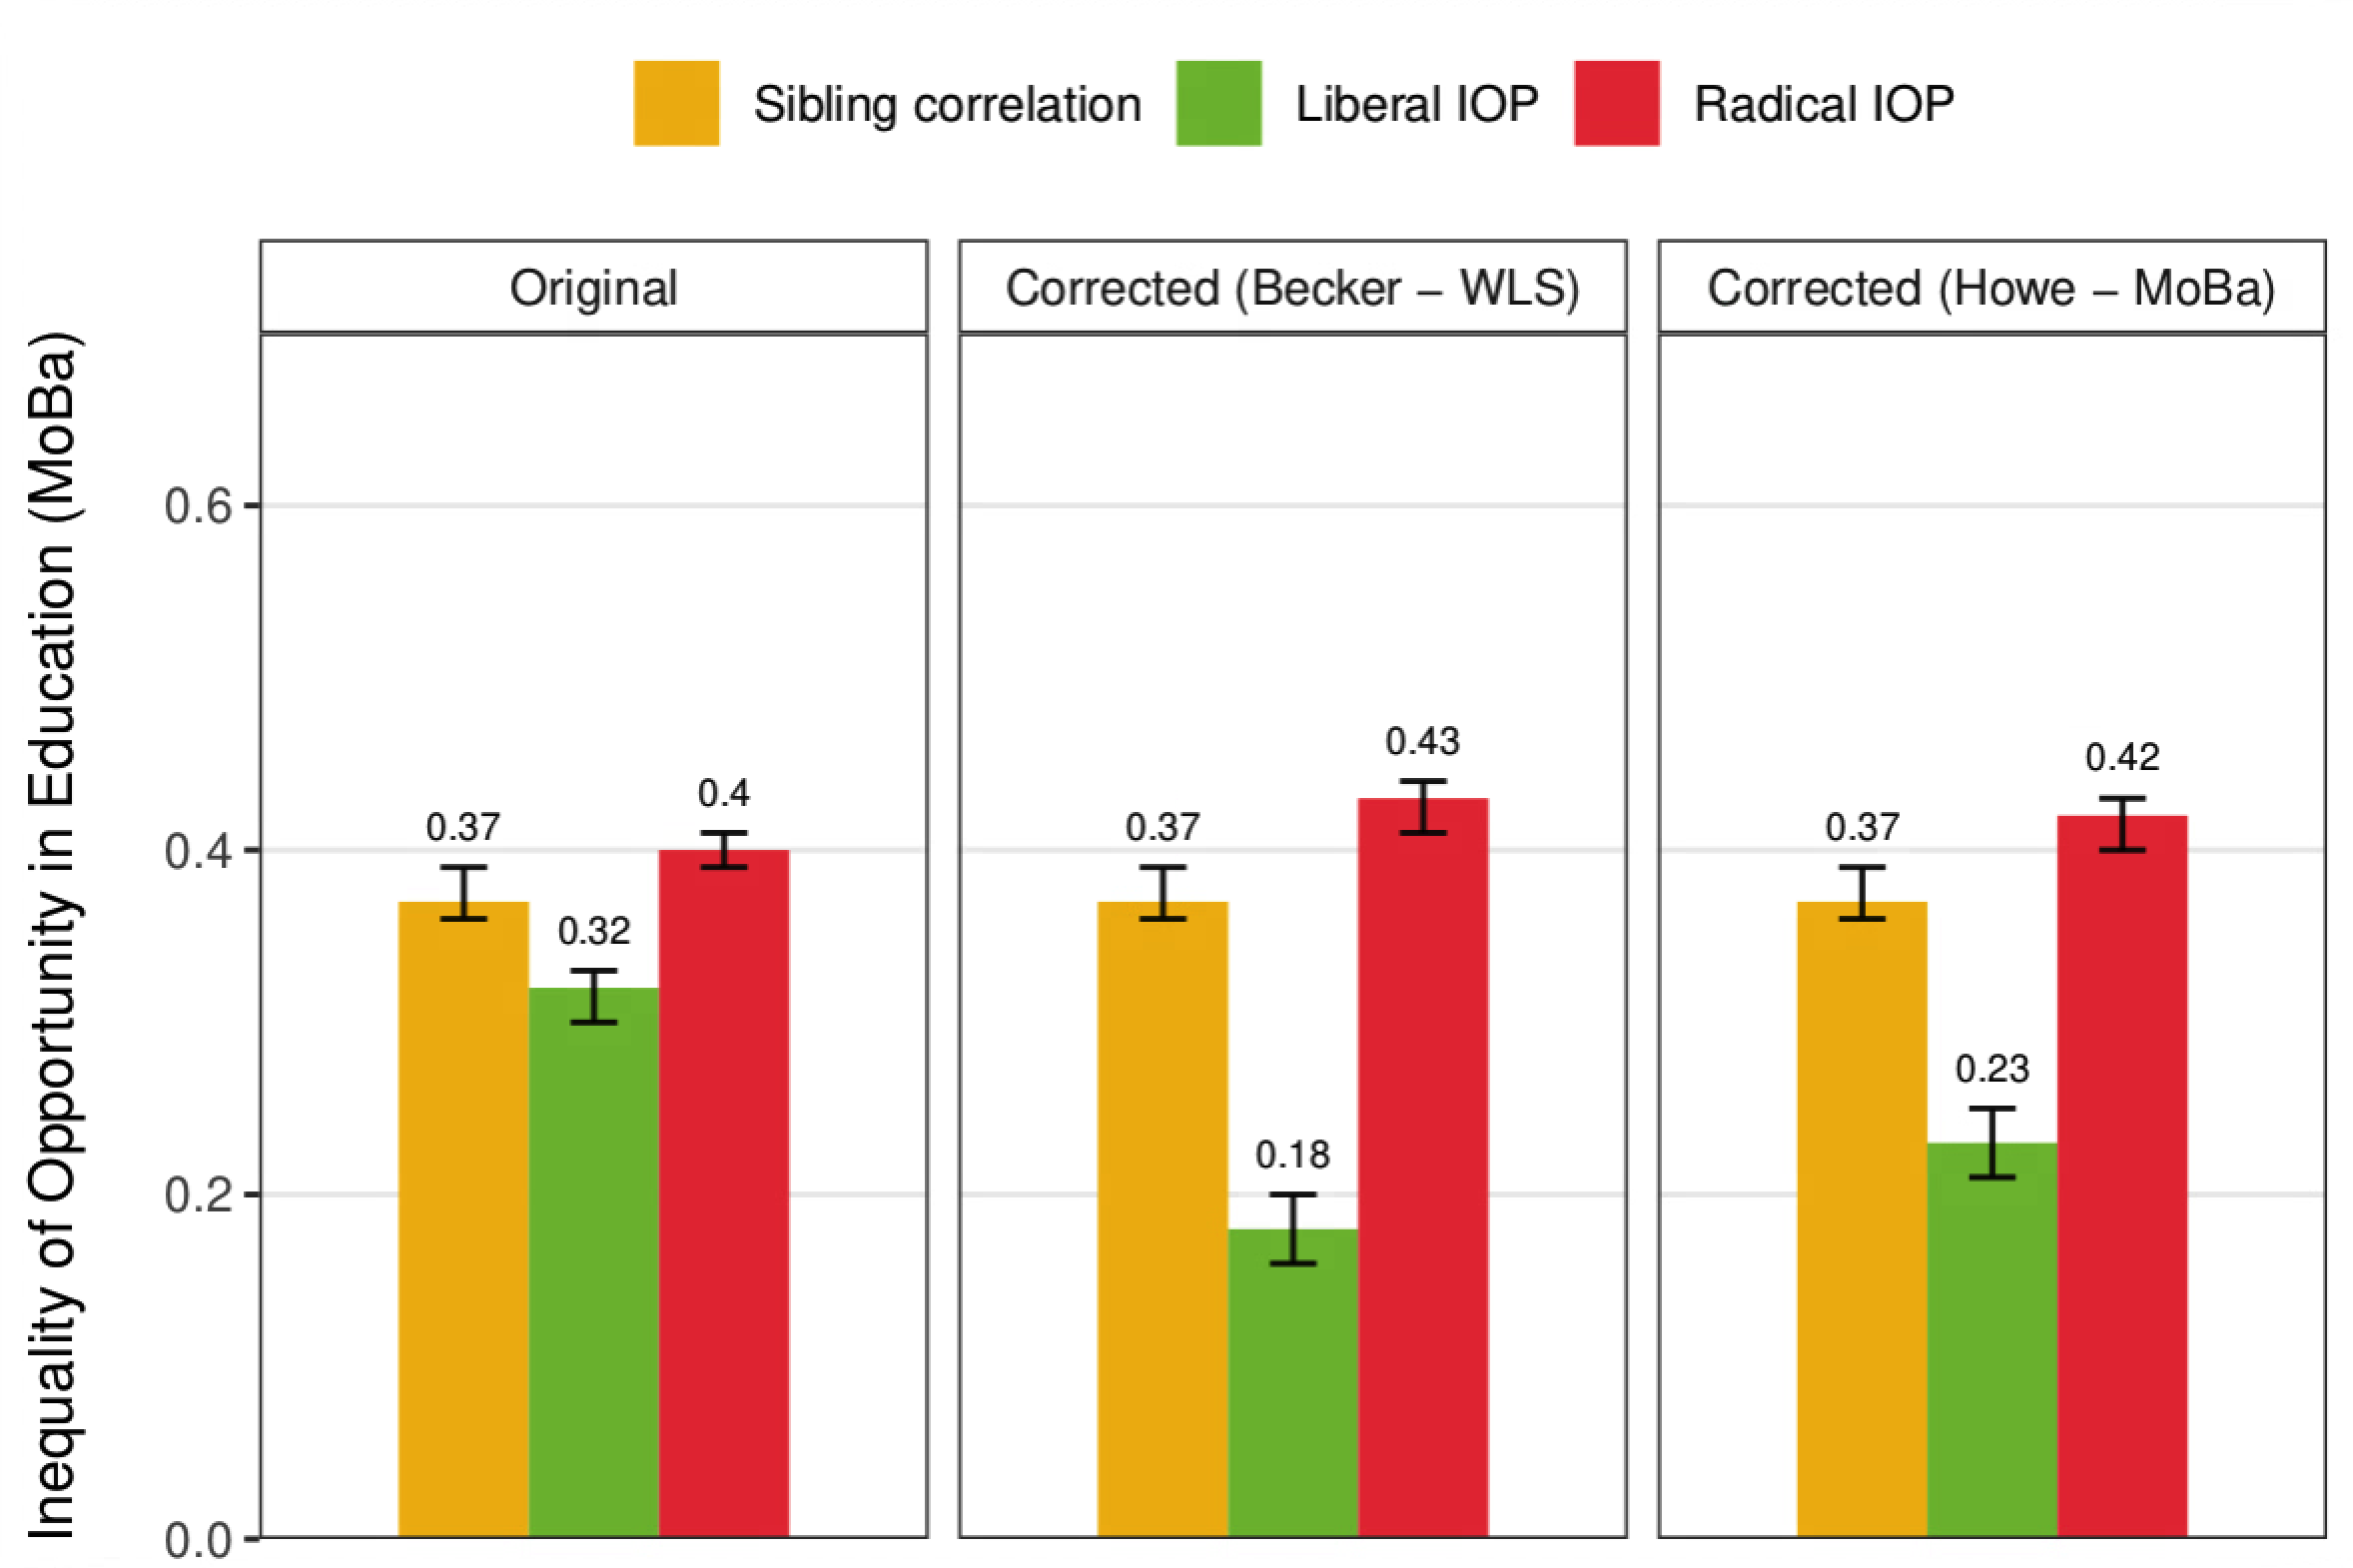
\includegraphics[keepaspectratio,alt={MoBa correction}]{plots/PGI_RC_correction_MoBa.png}}
\caption{MoBa: corrected indices}
\end{figure}

\begin{table}[H]
\begin{tabular}{@{}lcccccccc@{}}
\toprule
 & $h^2_\text{between}$ & $h^2_\text{within}$ & $\rho_\text{between}$ & $\rho_\text{within}$ & Sibcorr & IOLib & IORad & Gap \\
\midrule
Original & --- & --- & --- & --- & 0.37 & 0.32 & 0.40 & 0.08 \\
Corrected (Becker -- WLS) & 0.119 & 0.053 & 1.752 & 1.975 & 0.37 & 0.18 & 0.43 & 0.25 \\
Corrected (Howe -- MoBa) & 0.090 & 0.040 & 1.523 & 1.717 & 0.37 & 0.23 & 0.42 & 0.19 \\
\bottomrule
\end{tabular}
\end{table}

\emph{MoBa data parameters: \(R^2_\text{between} = 0.104\),
\(R^2_\text{within} = 0.022\), ICC \(= 0.374\),
\(R^2_\text{pop} = 0.052\).}



\subsection{\texorpdfstring{Check: single-\(\rho\) vs.~decomposed
correction}{Check: single-\rho vs.~decomposed correction}}

The decomposed correction (\(\rho_\text{between}\),
\(\rho_\text{within}\) separately) used to compute the corrected version
of each index should be consistent with a check where a single
\(\rho_\text{pop}\) scales the radical-liberal gap, accounting for the
total genetic contirbution (between and within families):

\[\text{IORad}_\text{RC} - \text{IOLib}_\text{RC} = \rho^2_\text{between}\,\Delta_\text{between} + \rho^2_\text{within}\,\Delta_\text{within} = \rho^2_\text{pop}\,\Delta_\text{observed}\]

Single \(\rho_\text{pop}\) is either: 

\begin{itemize}
  \item implied from the data, using \(h^2_\text{pop}\) values reported in Becker et al (2021) and in Howe et al (2022)
  \item taken as directly reported in Becker et al (2021)
\end{itemize}


The gap check validates the decomposed correction. In \textbf{WLS} the
decomposed Becker result (0.24) matches Becker's directly reported
\(\rho = 1.649\) exactly, and is close to the implied single-\(\rho\)
value (0.23). The Howe decomposed result (0.18) is also close to the
Howe single-\(\rho\) check (0.17). This internal consistency confirms
that the between/within decomposition of \(\rho\) is coherent with the
population-level estimate.

In \textbf{MoBa} the match is looser for Becker: the decomposed result
(0.24) sits between the reported single-\(\rho\) (0.21) and the implied
single-\(\rho\) from our \(R^2_\text{pop}\) (0.26). The Howe decomposed
result (0.18) matches the Howe single-\(\rho\) (0.19) closely. The small
discrepancy for Becker in MoBa reflects the fact that Becker's \(h^2\)
estimate is WLS-specific and the \(R^2\) is estimated in MoBa,
introducing a cross-study mismatch for that scenario.

\begin{figure}
\centering
\pandocbounded{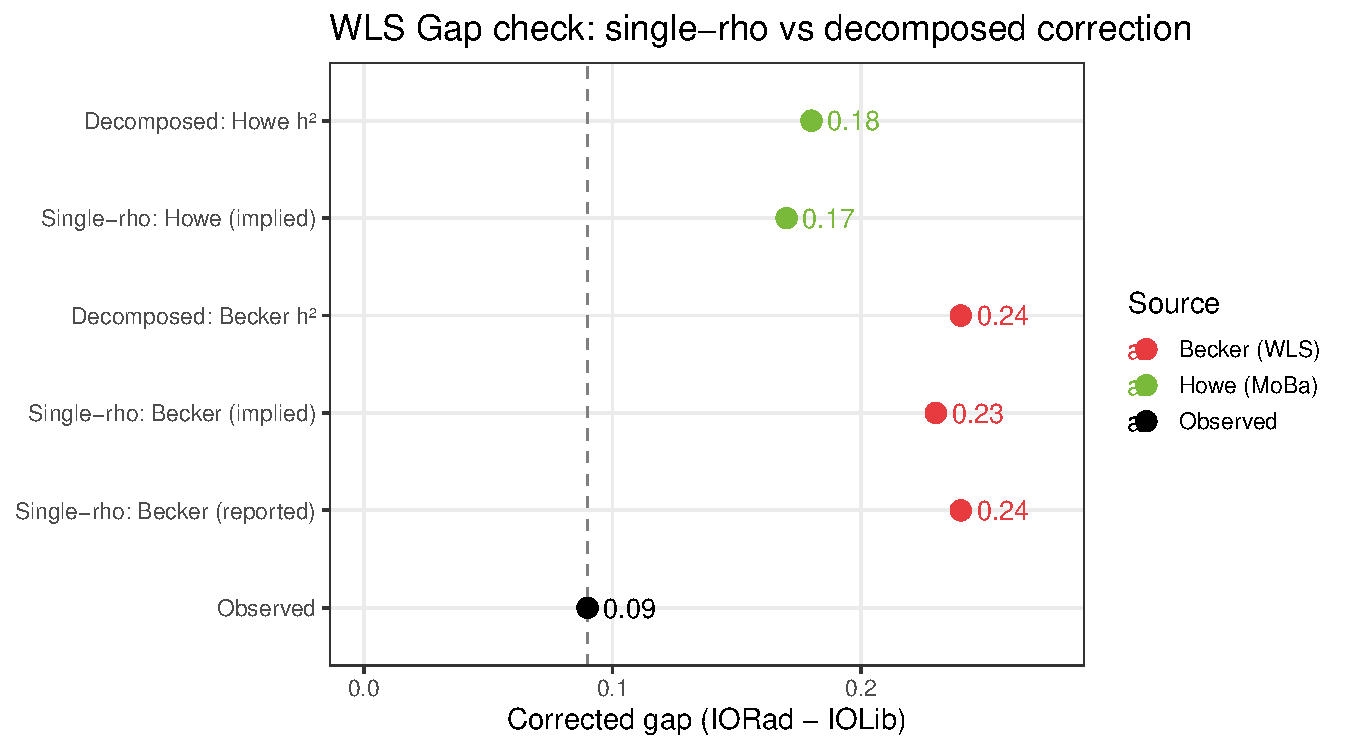
\includegraphics[width=0.7\textwidth]{plots/PGI_RC_gap_check_WLS.pdf}}
\caption{WLS: decomposition check}
\end{figure}


\begin{figure}
\centering
\pandocbounded{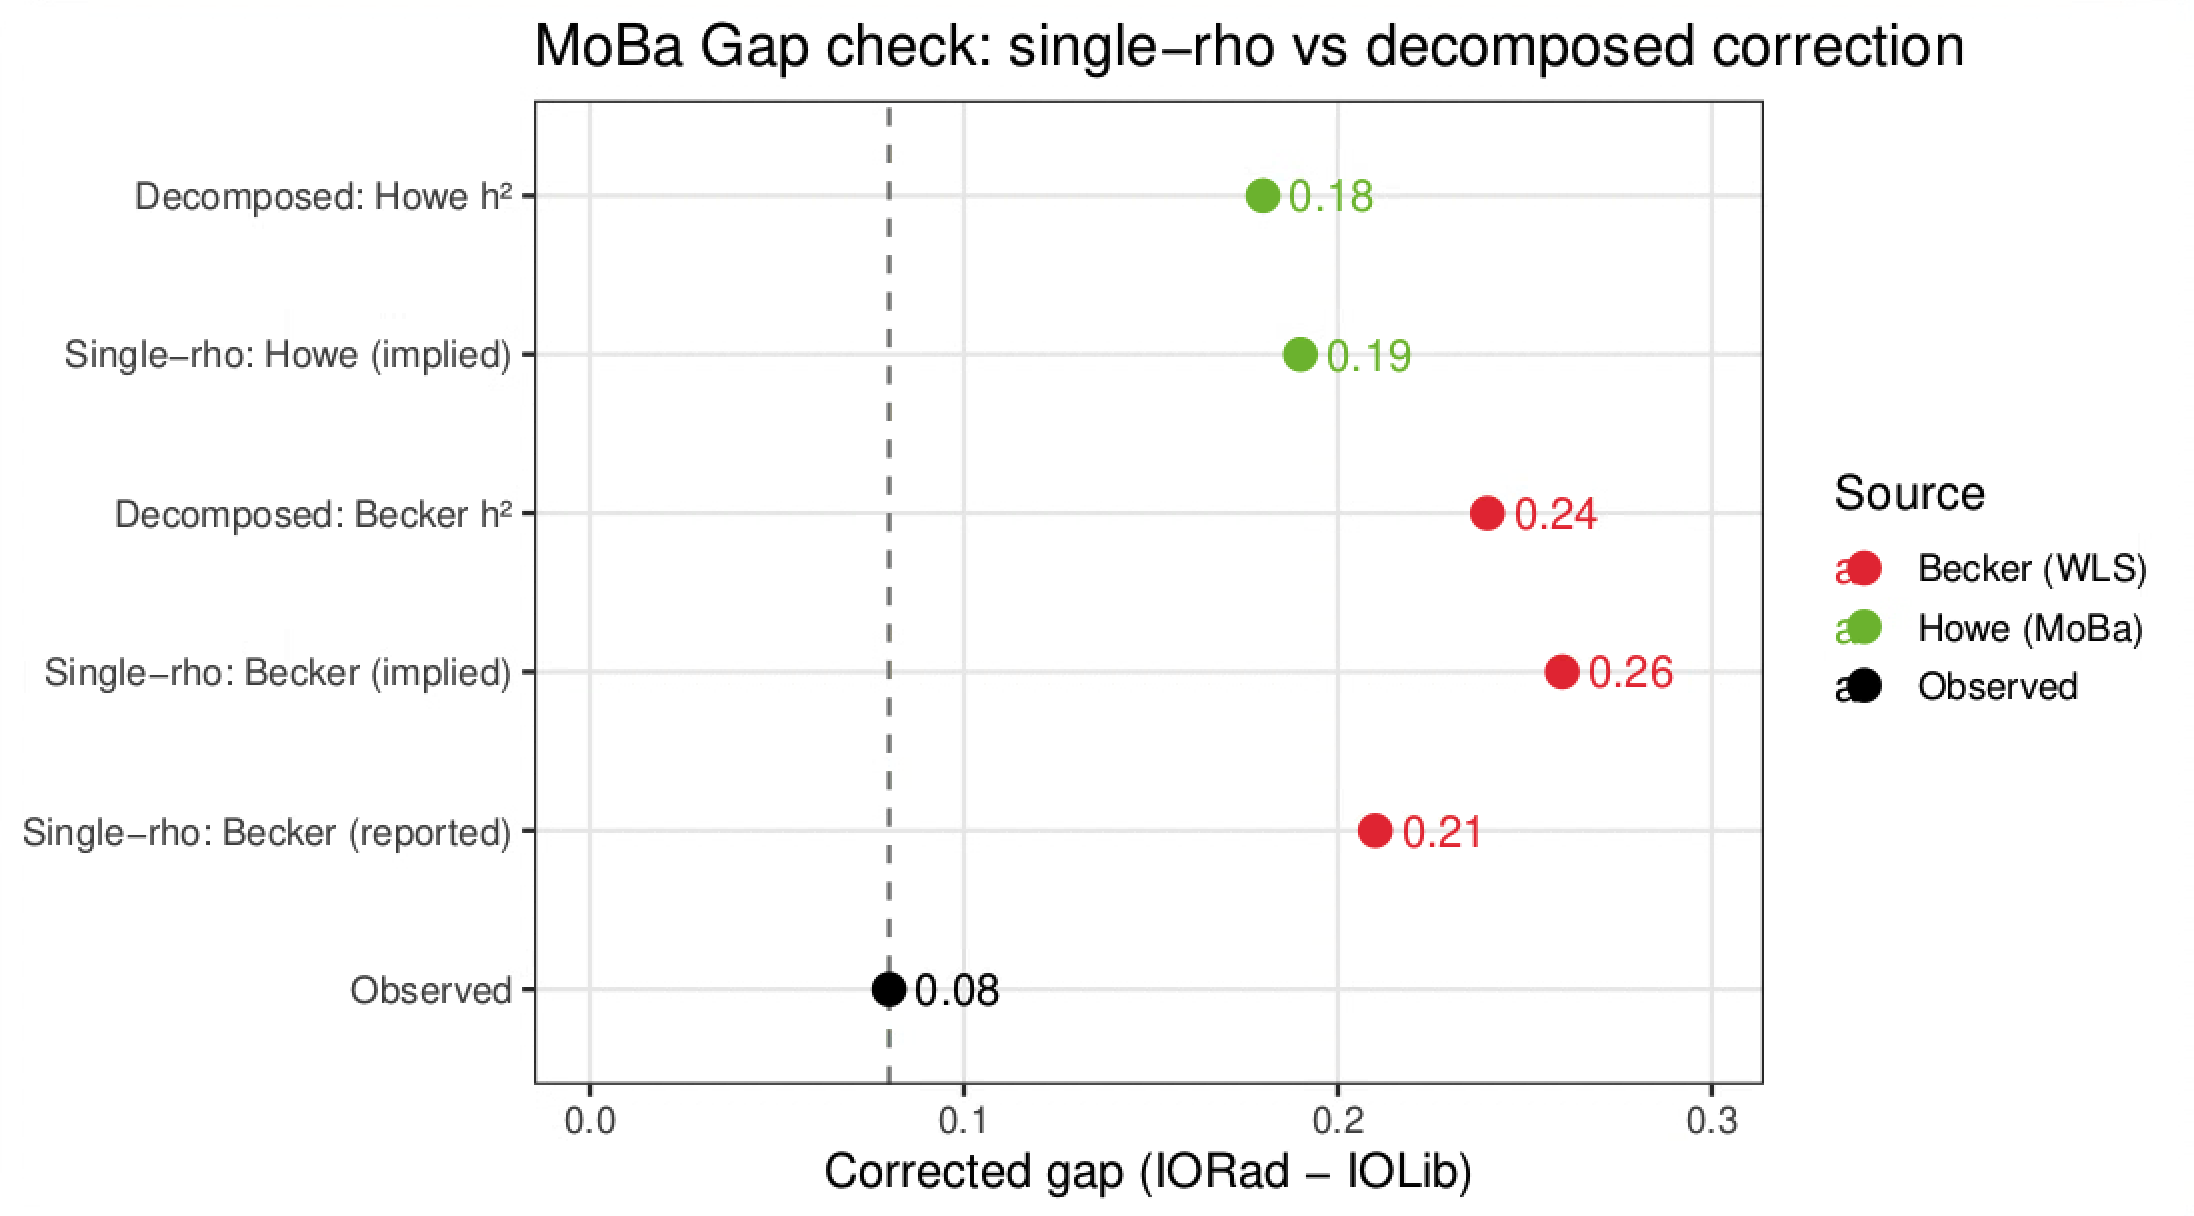
\includegraphics[width=0.7\textwidth]{plots/PGI_RC_gap_check_MoBA.png}}
\caption{MoBa: decomposition check}
\end{figure}


\end{document}
